\documentclass[11pt,a4paper]{article}
\usepackage[T1]{fontenc}\usepackage[utf8]{inputenc}\usepackage{lmodern}
\usepackage[margin=24mm]{geometry}\usepackage{amsmath,amssymb,booktabs,graphicx,tabularx,microtype}
\usepackage{array,enumitem,xcolor,longtable}
\usepackage[hidelinks]{hyperref}\usepackage{caption,placeins}
\captionsetup{font=small,labelfont=bf}\setlength{\emergencystretch}{2em}
\newcommand{\ind}{\mathbf 1}
\newcolumntype{Y}{>{\raggedright\arraybackslash}X}
\title{Intermittency-aware graph residual boosting for selective back-order prediction in multi-echelon supply chains}
\author{}\date{}
\begin{document}\maketitle
\begin{abstract}
Network context can improve shortage forecasts when upstream and neighboring states carry information absent from a focal node, but indiscriminate graph aggregation can add noise under intermittent demand. We propose intermittency-aware graph residual boosting (IGRB), a two-expert procedure for two-cycle back-order occurrence and severity. A local boosted expert is fitted first. A topology-aware expert uses causal histories of the focal node, parent, children, siblings and network aggregate. Validation selects a logit-space residual blend, while an average inter-demand interval screen can reject graph correction in sparse regimes. A separate guardrail activates emergency replenishment only after consistent validation-cost improvement. Evaluation uses a material-conserving three-echelon simulator, three synthetic regimes, retail-derived traces, two operational shifts, five model seeds and up to ten independent demand replications. Across ten unchanged correlated-demand replications, IGRB improves macro F1 over its local expert by 0.0269 (95\% paired bootstrap interval 0.0080--0.0436; nine wins). The seasonal mean gain is 0.0033 and its interval crosses zero; intermittent demand deliberately returns to the local expert. In the fixed realization IGRB exceeds the strongest previously evaluated method in three cases and is practically tied in the retail-driven case. In closed loop, the guardrail abstains in three cases; in correlated demand, IGRB reduces mean cost under all conditions. The evidence supports selective use of network context rather than universal graph-model superiority.
\end{abstract}
\noindent\textbf{Keywords:} back-order prediction; multi-echelon supply chain; graph features; gradient boosting; intermittent demand; distribution shift.

\section{Introduction}
Back orders emerge from coupled operational states. A terminal can become short because its own demand increases, an upstream node is constrained, a sibling competes for supply, or deliveries are delayed. Supply networks are natural candidates for graph-based forecasting. Yet network structure is not uniformly useful: local history may already summarize the relevant signal, and aggregation can amplify noise when demand is sparse. The industrial question is not simply whether a graph model can be fitted, but when network context should be trusted and when a system should return to a strong local model.

This distinction matters because a back order is neither an ordinary demand observation nor a purely local response. It is an endogenous consequence of demand, inventory position, outstanding orders, allocation, capacity and transit time. Two terminals with identical recent demand can therefore have different shortage risks if their parents have different inventories or if their siblings compete differently for a constrained shipment. Conversely, a large relational model can be unnecessary when a terminal's recent inventory trajectory already contains the relevant information. A useful industrial predictor must negotiate both possibilities without assuming in advance that topology is always beneficial.

The forecasting target is also operationally asymmetric. Missing an imminent shortage can create backlog cost and poor service, while excessive warnings may trigger expensive emergency replenishment. Ranking and calibration both matter, but neither guarantees that an intervention lowers cost. A model may improve macro F1 by correcting borderline cases yet worsen positive shortage quantities; a policy driven by those quantities may then spend more despite the classification gain. We therefore treat occurrence prediction, conditional severity estimation and closed-loop intervention as related but distinct levels of evidence.

Classical multi-echelon theory studies coordinated stocking decisions \cite{clark,graves}. Prediction addresses a different layer: estimation of future shortage risk from observed states. Statistical improvement need not lower inventory cost because probabilities, quantities, intervention capacity and timing interact. Decision-focused learning makes this mismatch explicit \cite{spo,trees,mandi}; a forecasting contribution should therefore establish predictive value and the limits of downstream use.

Graph neural networks offer relational inductive biases \cite{gcn,rgcn,gat}, and recent supply-chain studies combine graphs with forecasting or control \cite{chang,kotecha}. Our preliminary benchmark found that a relation-aware neural model did not consistently beat tuned tabular and recurrent alternatives. We consequently preserve a competitive local predictor, add network information as a residual expert, and permit validation to reject that correction.

This redesign responds to a common failure mode in applied graph learning: a complex architecture is compared with weak or poorly tuned local baselines, and any advantage is attributed to graph reasoning. Here both local and graph-context experts use the same boosting family and optimization budget. Their difference is the information set. The graph expert is not allowed to replace the local expert automatically; it supplies a correction whose strength is chosen on a chronological validation block. A pre-specified intermittency screen can eliminate the correction, and a second validation gate separately decides whether predictions may drive emergency action. These safeguards make a tie informative: it records an explicit decision not to use relational evidence rather than a failed attempt to force it into every regime.

We propose intermittency-aware graph residual boosting (IGRB) and ask: (RQ1) when does causal network context improve back-order forecasts beyond a tuned local-history expert? (RQ2) does improvement persist across independent demand realizations and operational shifts? (RQ3) do forecast improvements translate into lower cost under a capacity-limited emergency rule?

The study contributes (i) a graph-context expert added as a validation-selected residual correction to a strong local expert; (ii) a transparent intermittency screen that can return exactly to the local expert; (iii) separate evaluation of model-seed and independent demand-realization variation, with component ablations; and (iv) a guarded closed-loop experiment that reports negative operational findings rather than inferring decision value from F1. The claim is a selective forecasting procedure and its empirical characterization, not a new inventory policy or universal superiority of graph learning.

The remainder of the article first positions the work at the intersection of multi-echelon inventory, intermittent-demand forecasting, spatiotemporal graph learning and decision-aware prediction. It then formalizes the simulator and information timing, describes IGRB and its two safeguards, and reports fixed-realization, independent-replication, shift, ablation and closed-loop results. The final sections distinguish conclusions supported by the evidence from questions that require observed industrial back-order records.

\section{Related work}
\subsection{Multi-echelon forecasting and decisions}
Clark and Scarf \cite{clark} and Graves and Willems \cite{graves} provide foundations for multi-echelon coordination and safety-stock placement. Their objective is operational cost under stated assumptions. Our setting retains a fixed order-up-to system and predicts future back-order states. Smart predict-then-optimize and related approaches incorporate downstream objectives into learning \cite{spo,trees,mandi}. IGRB instead separates prediction from a validation-guarded deployment rule, diagnosing whether predictive gains survive a closed loop.

Forecasting and inventory control are coupled but non-equivalent tasks. Forecast accuracy measures summarize errors in an information product; an inventory objective additionally depends on lead time, review timing, capacity, order rules and the relative costs of stock, shortage and intervention. Classical work therefore warns against choosing forecasts solely by generic accuracy when the ultimate use is inventory control \cite{gardner,kolassa}. In multi-echelon systems the mapping becomes still less direct because an action at one node changes the future state and information available elsewhere. Our experiment holds the baseline order-up-to policy fixed and asks a narrower question: whether a shortage forecast can safely augment that policy through a capacity-limited emergency channel.

Decision-focused learning embeds an optimization problem in training or uses regret-sensitive surrogates \cite{spo,trees,mandi}. That approach can be powerful when the downstream problem and cost parameters are trusted. Our costs are intentionally stylized, so end-to-end decision training would risk making the predictor appear precise only for one assumed scenario. Instead, the occurrence and severity models are trained predictively, while a validation guardrail determines whether the downstream action is authorized. The design sacrifices claims of policy optimality in exchange for a transparent separation between forecasting evidence and operational evidence.

\subsection{Graph learning and tabular experts}
Graph convolution, relational convolution and graph attention aggregate neighboring information \cite{gcn,rgcn,gat}. XGBoost remains a strong alternative for structured histories because it captures nonlinear interactions without end-to-end representation learning \cite{xgb}. We use boosting for both experts so the comparison isolates information structure and residual selection rather than neural-versus-tree optimization. The method resembles stacking, but its safeguards are central: chronological blend selection, an intermittency screen and exact fallback.

Spatiotemporal graph architectures have been successful when variables are linked by stable physical or functional relations. Diffusion convolutional recurrent networks combine directed diffusion with recurrent dynamics \cite{dcrnn}; STGCN couples graph convolution with temporal convolution \cite{stgcn}; Graph WaveNet learns adaptive dependencies in addition to a specified graph \cite{graphwavenet}; and MTGNN learns graph structure for multivariate time series \cite{mtgnn}. These models motivate relational temporal learning, but transport and sensor benchmarks differ from an inventory network in two respects. First, shortage is generated by a controlled stock-flow system rather than observed continuously as a physical signal. Second, zeros can represent genuine inactivity rather than missing information. Indiscriminate message passing can consequently smooth together incompatible states or amplify sampling noise.

Tree ensembles provide a demanding baseline for this setting. They handle nonlinear thresholds, interactions, heterogeneous scales and mixed temporal summaries with comparatively little representation tuning. Forecasting competitions have repeatedly shown that combinations and strong statistical or boosted baselines remain difficult to displace across heterogeneous series \cite{m4,m5}. The purpose of using the same XGBoost family for both experts is therefore experimental control: improvement can be attributed to parent, child, sibling and network context rather than to a larger neural architecture or a different optimizer.

Modern global forecasting models provide another relevant comparison. DeepAR learns probabilistic autoregressive models across related series \cite{deepar}; N-BEATS uses interpretable or generic residual blocks \cite{nbeats}; and the Temporal Fusion Transformer combines recurrent processing, variable selection and attention \cite{tft}. These methods can share statistical strength without an explicit supply topology. IGRB addresses a different, narrower hypothesis: whether known operational roles add incremental signal beyond a tuned local history in a small network. A broader empirical study should compare both kinds of sharing under equal tuning budgets.

Residual combination has a related motivation. Forecast combinations often reduce risk because component errors are imperfectly correlated \cite{batesgranger,clemen}. IGRB differs from an unconstrained ensemble: the local expert is the reference, the graph expert is expressed as a correction in logit or quantity space, and zero correction is an admissible and operationally meaningful solution. This nested construction supports an exact fallback that ordinary averaging does not provide.

\subsection{Intermittent demand}
Intermittent demand requires attention to spacing and size of nonzero observations. Syntetos, Boylan and Croston use average inter-demand interval (ADI) and squared coefficient of variation to categorize demand \cite{syntetos}. Their ADI boundary of 1.32 distinguished behavior of Croston-type estimators; it is not a universal machine-learning threshold. We use 1.32 only as a pre-specified heuristic screen and test its role by ablation.

Croston's method separately updates nonzero size and inter-arrival interval \cite{croston}; later corrections address bias and obsolescence \cite{sba,tsb}. This literature establishes that the timing of zeros changes which information is useful. It does not imply that a Croston-type point forecast is sufficient for a network back-order target, because shortage also depends on stock and replenishment. We borrow only the diagnostic idea that sparse arrival timing should influence model selection. The median terminal ADI is easy to audit, uses training data only and creates a falsifiable rule: if the threshold is removed, graph use should be evaluated explicitly.

Our contribution relative to these streams is thus not a new universal graph neural network. It is a selective architecture for an operational target: a competitive local expert is augmented only when relational histories provide validated incremental information, and even a validated predictive correction cannot trigger action without separate cost evidence. Table~\ref{tab:positioning} summarizes the resulting gap.

\begin{table}[tb]\centering\small
\caption{Positioning of the study relative to adjacent methodological streams.}\label{tab:positioning}
\begin{tabularx}{\linewidth}{p{.19\linewidth}YYY}\toprule
Stream & Primary strength & Limitation for the present question & Element adopted here \\\midrule
Multi-echelon inventory & Coordinated stock and service decisions & Usually assumes a demand model rather than learning shortage risk from state histories & Material-conserving controlled network and explicit cost accounting \\
Intermittent-demand forecasting & Separates nonzero size and arrival spacing & Mainly local demand; does not represent upstream competition & Training-only ADI as a graph-use screen \\
Spatiotemporal GNNs & Encodes linked temporal variables & Message passing can be high variance and difficult to justify on small sparse networks & Causal role-based graph summaries \\
Decision-focused learning & Aligns prediction with downstream loss & Sensitive to the assumed optimization problem and cost parameters & Separate validation cost guardrail \\
Forecast combination & Diversifies model error & Unconstrained averaging cannot guarantee fallback & Nested residual blend with $\alpha=0$ \\
\bottomrule\end{tabularx}
\end{table}

\section{Inventory system and prediction task}
\subsection{Network dynamics}
The controlled network is a rooted three-echelon tree with one supplier, three distribution nodes and twelve terminals. Fifteen material edges point downstream and fifteen information edges upstream. Scheduled arrivals occur first. Terminals serve customer demand and backlog; internal nodes allocate stock proportionally to pending child orders. New orders are placed before the parent is processed, dispatched material enters the child's pipeline, and unsatisfied orders remain pending.

Figure~\ref{fig:topology} distinguishes the two directed relations. Downstream edges carry physical material and allocation effects; upstream edges carry orders and state information. The roles are not interchangeable. A terminal's parent summarizes immediate replenishment availability, its siblings represent competition for that availability, and the terminal aggregate represents system-wide demand pressure. These operational roles determine the graph-context features used later; no feature is obtained by looking ahead in the simulated trajectory.

\begin{figure}[tb]\centering
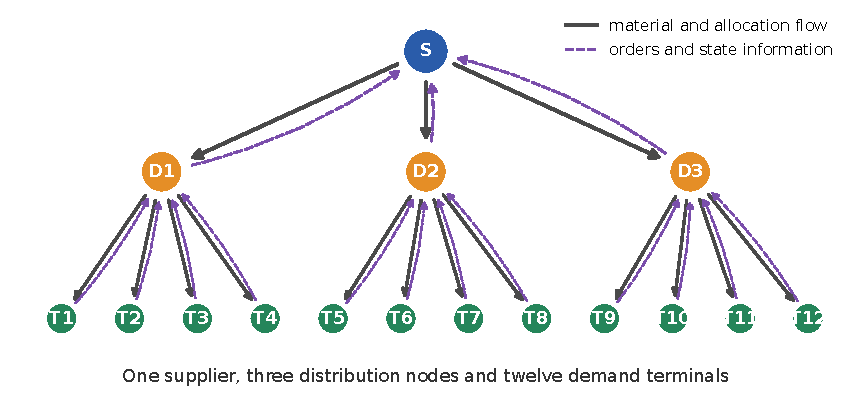
\includegraphics[width=.96\linewidth]{igrb_topology.pdf}
\caption{Three-echelon experimental network. Solid arrows denote downstream material/allocation flow; dashed arrows denote upstream orders and information. Graph-context features preserve these operational roles rather than treating the graph as homogeneous.}\label{fig:topology}
\end{figure}

Let $I_{v,t}$ denote end-of-cycle stock, $B_{v,t}$ unserved outgoing demand and $D_{v,t}$ new demand. With pre-service stock $I^-_{v,t}$ and capacity $C_{v,t}$,
\begin{align}F_{v,t}&=\min\{I^-_{v,t},B_{v,t-1}+D_{v,t},C_{v,t}\},\\
I_{v,t}&=I^-_{v,t}-F_{v,t},\qquad B_{v,t}=B_{v,t-1}+D_{v,t}-F_{v,t}.
\end{align}
The order-up-to target is $S_v=\mu_v(L+1)+\sigma_v\sqrt{L+1}$ with nominal transit time $L=2$. A node orders
\begin{equation}Q_{v,t}=\left[S_v-\{I_{v,t}+P_{v,t}+U_{v,t}-B_{v,t}\}\right]_+,
\end{equation}
where $P$ is dispatched inbound supply and $U$ is ordered but not dispatched. Normal capacity is $1.6\mu_v$; a node-cycle disruption occurs with probability 0.04 and reduces capacity to one quarter. The simulator checks physical conservation after every cycle: cumulative external receipts plus initial stock equal current stock, customer service and internal-transit material, within numerical tolerance.

The within-cycle event order is fixed to prevent ambiguous timing. At the start of a cycle, shipments scheduled for that cycle enter on-hand stock. Terminals next serve accumulated customer backlog and new demand; internal nodes then observe child orders and allocate available capacity proportionally when total requested quantity exceeds supply. A dispatch reduces parent inventory immediately and enters a dated pipeline for the child. After service and allocation, every non-source node places a replenishment order using its inventory position. The source receives an external replenishment so that material entering the modeled boundary is recorded explicitly. Changing this order would change both labels and which features are admissible, so the implementation stores event ledgers and tests the timing invariants.

The order-up-to formula is a controlled experimental rule, not an estimated optimal policy. Its $(L+1)$ coverage reflects the review cycle plus nominal transit time, and the square-root term provides a common safety factor. Pending but undispatched orders $U$ are separated from dispatched pipeline stock $P$ because parent capacity can delay the former without violating material conservation. Backlog is carried forward rather than converted to lost sales. These assumptions create network dependence through competition and delay while keeping the source of each shortage traceable.

\begin{table}[tb]\centering\small
\caption{Inventory-system parameters held fixed unless a named shift is applied.}\label{tab:system}
\begin{tabularx}{\linewidth}{p{.30\linewidth}p{.20\linewidth}Y}\toprule
Quantity & Value & Interpretation \\\midrule
Network & $1+3+12$ nodes & Supplier, distribution and terminal echelons \\
Forecast horizon & 2 cycles & Back-order state and normalized quantity at $t+2$ \\
History length & 6 cycles & All model inputs end at forecast origin $t$ \\
Nominal transit time & $L=2$ & Increased to 3 only in the lead-time shift \\
Normal service capacity & $1.6\mu_v$ & Node-specific mean-demand scaling \\
Disruption probability & 0.04 per node-cycle & Capacity becomes 25\% of normal \\
Order-up-to shift & $0.65S_v$ & Applied only at the test boundary in the policy shift \\
Emergency capacity & $0.15\sum_{v\in\mathcal V_{\rm term}}\mu_v$ & Shared terminal intervention budget \\
Cost coefficients & 0.1, 5, 2 & Holding, terminal backlog and emergency receipt \\
\bottomrule\end{tabularx}
\end{table}

\subsection{Targets and causal inputs}
At the end of cycle $t$, the model predicts
\begin{equation}y_{v,t+2}=\ind[B_{v,t+2}>10^{-6}],\qquad b_{v,t+2}=B_{v,t+2}/\mu_v.
\end{equation}
The local vector contains six cycles of normalized on-hand stock, backlog, demand, nominal lead time, replenishment order and service fraction, plus deterministic time coordinates. Scaling moments use only training. Every input is available by the end of $t$; no future state enters preprocessing or feature construction.

Occurrence and severity are modeled separately because zeros dominate some cases and because the cost of a positive shortage depends on its size. The conditional severity target is trained only where $y=1$; at prediction time the occurrence probability and nonnegative severity estimate remain separate outputs. This design avoids forcing a single squared-error objective to explain both whether a shortage occurs and how large it is. It also allows the closed-loop policy to rank by occurrence risk while scaling quantities by predicted severity.

Normalization by the training mean $\mu_v$ makes node quantities comparable without using validation or test information. Service fraction is fulfilled demand divided by demand available for service, with a defined value when the denominator is zero. Calendar coordinates are deterministic sine and cosine terms for the known simulation period or observed day index. No rolling statistic crosses a partition boundary in a way that exposes future observations. Table~\ref{tab:features} records the information sets so that ``graph context'' is operationally reproducible.

\begin{table}[tb]\centering\small
\caption{Causal feature construction at forecast origin $t$. Each dynamic block contains lags $t-5,\ldots,t$.}\label{tab:features}
\begin{tabularx}{\linewidth}{p{.22\linewidth}p{.31\linewidth}Y}\toprule
Block & Variables or operation & Purpose \\\midrule
Local state & On-hand, backlog, demand, lead time, order, service fraction & Strong node-specific reference information \\
Parent history & Same dynamic state at immediate supplier & Upstream availability and delay \\
Child mean & Mean history over direct children & Downstream pressure at internal nodes \\
Sibling mean & Mean history over nodes sharing a parent & Competition for constrained supply \\
Terminal mean & Mean history over all terminals & Common system demand pressure \\
Contrasts & Focal minus parent; focal minus sibling mean & Relative imbalance not visible in pooled levels \\
Time & Deterministic calendar coordinates & Seasonality without future observations \\
Missing role & Replace absent role by focal history & Fixed dimension without learned missing tokens \\
\bottomrule\end{tabularx}
\end{table}

\section{Intermittency-aware graph residual boosting}
\subsection{Local and graph-context experts}
The local expert uses an XGBoost classifier $p^L_{v,t}$ and a positive-only severity regressor $q^L_{v,t}$. Depth is selected from $\{3,6\}$ on chronological validation. For each node, the graph-context vector concatenates six-cycle histories of (i) the focal node, (ii) its parent, (iii) mean children, (iv) mean siblings, and (v) mean terminals, plus focal-minus-parent and focal-minus-sibling contrasts. Missing roles use the focal history to keep dimension fixed. These are causal summaries of the known tree, not learned embeddings. A second classifier and regressor, with depth in $\{2,4\}$, form $(p^G,q^G)$.

Both experts use 180 trees, learning rate 0.05, row subsampling 0.9, feature subsampling 0.85, minimum child weight two and $L_2$ regularization two. Occurrence models use all node--cycle targets; severity models use positive targets only. Settings, candidates and predictions are retained.

Let $x^L_{v,t}$ denote the local vector and $x^G_{v,t}$ the concatenated role-based vector. The two classifiers approximate
\begin{equation}
p^L_{v,t}=P(y_{v,t+2}=1\mid x^L_{v,t}),\qquad
p^G_{v,t}=P(y_{v,t+2}=1\mid x^L_{v,t},x^G_{v,t}),
\end{equation}
while $q^L$ and $q^G$ approximate $E[b_{v,t+2}\mid y_{v,t+2}=1,\cdot]$. Including $x^L$ in the graph expert is intentional: it asks whether contextual variables add information after the focal history is available. The comparison would be less informative if the graph expert were deprived of strong local predictors.

The role summaries are deterministic and low dimensional. They can be understood as one-step, typed aggregation with a fixed readout rather than a learned graph embedding. This choice follows from the small network and the earlier neural benchmark: adding message-passing capacity did not establish robust gains, whereas a controlled information-set comparison directly tests the industrial hypothesis. It also permits feature-level inspection and avoids a mismatch in which the proposed model receives more tuning simply because it has a more complex optimizer.

\subsection{Residual blend and abstention}
For $\alpha\in\{0,0.1,\ldots,1\}$,
\begin{align}p^{I}_{v,t}&=\sigma\!\left(\operatorname{logit}p^L_{v,t}+\alpha[\operatorname{logit}p^G_{v,t}-\operatorname{logit}p^L_{v,t}]\right),\\
q^{I}_{v,t}&=\max\{0,q^L_{v,t}+\alpha(q^G_{v,t}-q^L_{v,t})\}.
\end{align}
The classification threshold is selected from 141 equally spaced values between 0.15 and 0.85. Validation selects graph depth and $\alpha$ by maximizing
\begin{equation}\mathcal S=F_{1,\mathrm{macro}}+0.05\,\mathrm{AP}-0.02\,\mathrm{Brier}-0.03\,J_{\mathrm{proxy}}/J_{\mathrm{proxy}}^{L},\end{equation}
where the proxy ranks predicted terminal shortages under the emergency-capacity bound but does not alter simulator states. Coefficients and grids are fixed across cases. If the best graph candidate fails to improve the local score by $10^{-4}$, $\alpha=0$.

The median terminal ADI is
\begin{equation}\mathrm{ADI}=\operatorname{median}_{v\in\mathcal V_{\rm term}}\frac{T_{\rm cal}}{\sum_{t\leq T_{\rm cal}}\ind[D_{v,t}>0]}.
\end{equation}
If ADI exceeds 1.32, graph correction is disabled. This auditable safeguard is evaluated with a no-ADI ablation.

Logit interpolation is used for occurrence because the correction is then additive in log odds. At $\alpha=0$ the result is identically local; at $\alpha=1$ it is the graph expert; intermediate values shrink the contextual correction toward zero. Severity uses an analogous convex residual correction followed by a nonnegativity constraint. The same $\alpha$ is used for both heads to keep selection compact and to avoid presenting a large search as confirmatory evidence.

The validation score combines discrimination, calibration and a lightweight operational proxy. Macro F1 prevents the majority class from dominating, AP measures ranking without fixing a threshold, Brier score penalizes probability error, and the proxy discourages candidates that spend the emergency capacity on poor quantities. The coefficients do not have a claim of optimality. They were fixed before the confirmatory demand records and used unchanged for every case. A candidate must also exceed the local score by $10^{-4}$; this numerical margin prevents a negligible validation fluctuation from activating graph correction.

\begin{figure}[tb]\centering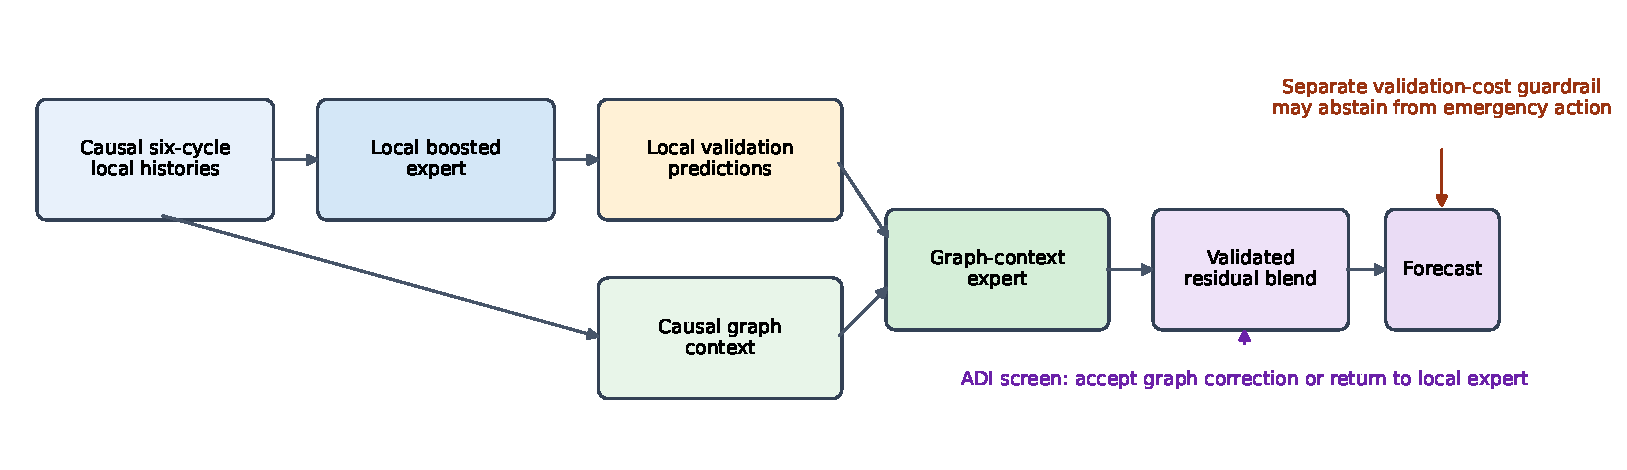
\includegraphics[width=.94\linewidth]{igrb_architecture.pdf}
\caption{IGRB workflow. A local expert and a causal graph-context expert are combined by a chronological validation-selected residual blend. An intermittency screen can return exactly to the local expert, while a separate cost guardrail may abstain from emergency action.}\label{fig:igrb}\end{figure}

\begin{table}[tb]\centering\small
\caption{Candidate set and fixed learning controls. Only the listed depth, blend, classification threshold and policy parameters are selected on validation.}\label{tab:hyper}
\begin{tabularx}{\linewidth}{p{.29\linewidth}p{.24\linewidth}Y}\toprule
Component & Candidate/value & Selection role \\\midrule
Local tree depth & $\{3,6\}$ & Chronological validation \\
Graph tree depth & $\{2,4\}$ & Chronological validation \\
Residual weight $\alpha$ & $0,0.1,\ldots,1$ & Joint validation score \\
Occurrence threshold & 141 values in $[0.15,0.85]$ & Validation macro F1 \\
Trees / learning rate & 180 / 0.05 & Fixed in all cases \\
Row / feature subsampling & 0.90 / 0.85 & Fixed regularization \\
Minimum child weight / $L_2$ & 2 / 2 & Fixed regularization \\
ADI boundary & 1.32 & Pre-specified screen; tested by ablation \\
Policy scale & retained candidates up to 0.25 & Validation cost, subject to guardrail \\
\bottomrule\end{tabularx}
\end{table}

\subsection{Training and selection protocol}
The procedure is deliberately nested around the local expert. First, local occurrence and positive-only severity models are trained for each local-depth candidate. Their validation predictions determine the reference score and threshold. Second, graph-context candidates are trained using the same rows and model seeds. For every graph depth and $\alpha$, blended validation predictions are constructed without refitting. The best admissible candidate is retained only if it clears the improvement margin and the ADI screen. Finally, the selected model and threshold are frozen for the test block and both operating shifts.

In compact form, the procedure is:
\begin{enumerate}[leftmargin=2.2em,itemsep=.15em]
\item Build training-only scaling statistics and six-cycle causal histories.
\item Fit local classifier/regressor candidates; select local depth and threshold on validation.
\item Fit graph-context classifier/regressor candidates on the same split.
\item Evaluate all $(\text{graph depth},\alpha)$ pairs using $\mathcal S$; compare the best score with the local reference.
\item Set $\alpha=0$ when the score margin is not cleared or median terminal ADI is above 1.32.
\item Freeze models, preprocessing, $\alpha$ and classification threshold; evaluate unchanged and shifted tests.
\item Independently search the emergency rule on validation and enable it only if the full block and both halves improve by at least 1\%.
\end{enumerate}

Steps 4 and 7 answer different questions. The former asks whether network context improves a predictive validation objective. The latter asks whether acting on the selected forecast improves a closed-loop cost. Conflating them would allow a small predictive gain to authorize an intervention even when its quantity errors or purchase costs are harmful.

\subsection{Decision guardrail}
A candidate policy ranks terminals by predicted risk and allocates a scaled predicted shortage subject to capacity $0.15\sum_{v\in\mathcal V_{\rm term}}\mu_v$. Thresholds and scales are selected on validation. Intervention is enabled only if total validation cost and the cost in each validation half improve by at least 1\%; otherwise no emergency action is taken. This prevents a statistically attractive forecast from automatically authorizing a costly decision.

At the end of cycle $t$, eligible terminals are sorted by $p_{v,t}$ with deterministic tie breaking. A terminal below the policy threshold receives zero; otherwise its request is the selected scale times $q_{v,t}\mu_v$, capped by remaining shared capacity. Emergency units arrive after the same two-cycle horizon used by the forecast. Because arrivals change future inventory, orders and backlog, every policy is simulated on its own trajectory and predictions are recomputed at each origin. Evaluation on a frozen no-action trajectory would overstate validity by ignoring feedback.

The half-block requirement guards against a policy whose apparent validation benefit comes entirely from a short favorable episode. It is not a statistical guarantee and may be conservative, especially with limited validation length. Its purpose is deployment discipline: absence of sufficiently stable cost evidence produces an explicit no-action decision. The predictive model can therefore be used for monitoring even when the intervention channel remains off.

\section{Evaluation design}
\subsection{Demand, partitions and shifts}
Three synthetic cases contain 480 cycles and twelve terminal streams. Seasonal demand uses Poisson rates with amplitude 0.35 and period 28. Intermittent demand combines Poisson sizes with Bernoulli occurrence probability 0.4. Correlated demand shares an autoregressive log-intensity factor. The retail-driven case contains 374 daily streams derived from UCI Online Retail \cite{uci}; only demand is empirical, while topology, inventory states and labels are simulated.

The cases are designed to vary the expected value of network context. Seasonal terminals share a deterministic calendar but retain node-specific Poisson variation, so global context may help modestly. Intermittent demand contains many genuine zeros; neighbor histories can be noisy and the ADI safeguard should be relevant. Correlated demand contains a latent common factor not supplied directly to the model, making contemporaneous upstream and sibling trajectories potentially informative. The retail-derived case tests irregular empirical demand shapes, but it is not an industrial back-order dataset: sales are transformed into terminal demand, and every inventory quantity remains generated by the simulator.

For the retail construction, transactions are aggregated by day and stock code, returns and nonpositive quantities are excluded, and twelve sufficiently active product streams are scaled to the terminal demand range. Transformation parameters are estimated from the training segment. The procedure preserves ordering and intermittent patterns but not customer identities, prices, cancellations or the original firm's replenishment process. This boundary is stated because referring to the case as ``real data'' without qualification would overstate external validity.

Records are split chronologically into 60\% training, 20\% validation and 20\% test. The primary benchmark fixes demand seed 101 and simulator seed 1001 and uses model seeds 11, 23, 37, 53 and 71. Independent records use seeds 202, 303, 404, 505 and 606; after finalizing the design, five confirmatory seasonal and correlated records use seeds 707, 808, 909, 1010 and 1111. Each set is paired with the five model seeds. Thus seasonal and correlated summaries contain ten independent records, while intermittent summaries contain five. Frozen models are also evaluated after two test-boundary shifts: transit time changes from two to three cycles, or order-up-to levels are multiplied by 0.65.

The distinction between model seeds and demand records is essential. Five model seeds on one record measure optimization and randomized tree variation conditional on the same demand, disruptions and labels. They do not quantify how the result changes when the supply chain experiences another demand realization. The paired record analysis therefore averages the five model seeds within each independently generated record and bootstraps the record-level differences. Seasonal and correlated cases receive five additional confirmatory records because they are precisely the regimes in which graph correction is activated. No result from those confirmatory records is used to modify the method.

Both shifts begin exactly at the test boundary. In the lead-time shift, new dispatches require three cycles while shipments already in transit retain their scheduled dates. In the policy shift, order-up-to targets fall to 65\% of their original values. Models, scalers, thresholds, blend weights and guardrail decisions remain frozen. These tests measure response to specific operating changes, not transfer to a new topology, supplier set or simulator family.

\begin{table}[tb]\centering\small
\caption{Evaluation cases and the expected informational role of graph context.}\label{tab:cases}
\begin{tabularx}{\linewidth}{p{.17\linewidth}p{.16\linewidth}p{.25\linewidth}Y}\toprule
Case & Length & Demand construction & Relational hypothesis \\\midrule
Seasonal & 480 & Poisson, period 28, amplitude 0.35 & Shared phase may create modest common signal \\
Intermittent & 480 & Bernoulli occurrence 0.4 with Poisson size & Sparse neighbor states may add variance; fallback expected \\
Correlated & 480 & Node demand driven by shared AR log intensity & Network histories proxy an omitted common driver \\
Retail-driven & 374 & Twelve scaled daily UCI product streams & Irregular empirical demand; all operational states simulated \\
\bottomrule\end{tabularx}
\end{table}

\subsection{Comparators, ablations and metrics}
The reconstructed benchmark contains persistence, a local balance score, pooled LSTM, mean and relational graph networks, graph-plus-GRU, homogeneous attention, relational attention plus GRU, the original relation-aware temporal GNN, and XGBoost. IGRB is compared directly with its tuned local expert. Graph-only and no-ADI controls test the principal components. An error-weighted expert is retained as a negative ablation because development experiments showed no consistent benefit.

Persistence carries the most recent shortage state forward. The balance score uses local stock, backlog and pipeline information without learned parameters. The pooled LSTM tests temporal memory without topology. Mean-GNN and relational-GNN alternatives test homogeneous and typed aggregation; graph-plus-GRU and relational-attention-plus-GRU add explicit temporal recurrence. The original HetST-GNN combines relation-aware aggregation with temporal conditioning and joint occurrence/severity heads. XGBoost uses local flattened histories. All reported ``previous best'' values come from this reconstructed benchmark; IGRB is not compared only with the rejected neural proposal.

The ablations answer four narrower questions. Local-only defines the exact fallback. Graph-only applies the contextual expert without residual protection. No-ADI allows validation to use a graph correction even in sparse regimes. Error-weighting upweights local mistakes when fitting the contextual expert. A component is supported only if its removal degrades relevant cases without creating a compensating advantage elsewhere; a single higher cell is not treated as proof.

We report macro F1 at the validation-selected threshold, average precision (AP), Brier score and positive-only severity RMSE. Independent-replication uncertainty uses a paired bootstrap over five demand realizations (20,000 resamples). Closed-loop cost is
\begin{equation}J=\sum_{t\in\mathcal T_{\rm test}}\left[0.1\sum_v I_{v,t}+5\sum_{v\in\mathcal V_{\rm term}}B_{v,t}+2\sum_v a_{v,t}\right].\end{equation}
Forecasts are recomputed from each policy's realized trajectory. Coefficients are stylized stress-test values, not measured monetary costs.

Macro F1 is the arithmetic mean of class-specific F1 values, which exposes performance on both shortage and non-shortage states under imbalance. AP evaluates risk ranking; Brier score is a proper score for the probability output \cite{brier}; RMSE$^+$ evaluates normalized quantity only on positive targets. These measures need not move together. In particular, better calibrated occurrence probabilities can coexist with worse positive severity, so the table reports both rather than collapsing them into a single success criterion.

For a paired record $r$, let $d_r=F1^{I}_r-F1^{L}_r$, after averaging its five model seeds. Percentile intervals resample the $n$ record indices with replacement 30,000 times and recompute $\bar d$. Pairing preserves the common demand and disruption sequence within a comparison. With only five or ten records, the interval remains coarse and should be read with the win--loss count, effect magnitude and shift consistency rather than as a binary publication threshold.

\subsection{Verification, reproducibility and claim control}
The simulator asserts nonnegative stock, backlog and allocations and verifies material conservation after every cycle. A future-demand mutation test confirms that changing demand after an origin does not change features at or before that origin. Scaling statistics and ADI are checked against training indices, and split construction enforces that the $t+2$ target remains inside its assigned partition. Shift tests verify identical pre-boundary trajectories. Closed-loop ledgers reconcile emergency requests, capacity, arrivals and cost components.

These checks follow the simulation principle that verification of implementation and validation of the conceptual model are separate activities \cite{sargent}. Conservation and mutation tests verify specific invariants; they do not validate the network as a representation of a particular firm. Likewise, the two shifts are controlled forms of distribution change, not a comprehensive concept-drift benchmark \cite{gama}.

The release retains configurations, seeds, split indices, trained candidate models, validation selections, per-node predictions, independent-record summaries, policy ledgers and the scripts that generate every reported table and figure. The fixed benchmark and independent records are separated in filenames to prevent model-seed variation from being mislabeled as data uncertainty. The historical archive named in the code statement predates this reconstruction and is not presented as reproducing the new results.

Three claim controls guide interpretation. First, ``retail-driven'' means empirical demand only, not observed inventory or shortage labels. Second, the independent-replication interval covers the specified simulator and demand generator, not an industrial population. Third, a lower simulated emergency cost demonstrates behavior under the stated coefficients and capacity, not an optimal replenishment policy. These qualifications are part of the experimental design rather than after-the-fact caveats.

\section{Results}Table~\ref{tab:primary} reports the fixed-realization comparison. IGRB selects nonzero graph corrections for seasonal and correlated demand and returns exactly to the local expert for intermittent and retail-driven demand. The graph contribution is selective by construction.
\begin{table}[tb]\centering\scriptsize
\caption{Unchanged-condition predictive results on the fixed benchmark realization (mean over five model seeds). RMSE$^+$ is normalized severity RMSE on positive targets.}\label{tab:primary}
\resizebox{\linewidth}{!}{\begin{tabular}{lrrrrrr}\toprule Case & Method & Macro F1 & AP & Brier & RMSE$^+$ & $\alpha$ \\\midrule
Seasonal & Local expert & 0.6752 & 0.4769 & 0.1138 & 0.4445 & 0.00 \\
Seasonal & IGRB & 0.6804 & 0.4852 & 0.1128 & 0.4415 & 0.68 \\
\addlinespace
Intermittent & Local expert & 0.6939 & 0.7902 & 0.1926 & 2.0331 & 0.00 \\
Intermittent & IGRB & 0.6939 & 0.7902 & 0.1926 & 2.0331 & 0.00 \\
\addlinespace
Correlated & Local expert & 0.7832 & 0.8801 & 0.1426 & 1.0458 & 0.00 \\
Correlated & IGRB & 0.7953 & 0.8899 & 0.1388 & 1.1139 & 0.52 \\
\addlinespace
Retail-driven & Local expert & 0.8611 & 0.9574 & 0.1047 & 8.6768 & 0.00 \\
Retail-driven & IGRB & 0.8611 & 0.9574 & 0.1047 & 8.6768 & 0.00 \\
\addlinespace
\bottomrule\end{tabular}}\end{table}
Figure~\ref{fig:fixed} visualizes the two occurrence metrics. In seasonal demand, the correction raises macro F1 by 0.0051 and AP by 0.0083 while slightly lowering Brier score and RMSE$^+$. In correlated demand, it raises macro F1 by 0.0120 and AP by 0.0098 and lowers Brier score by 0.0038, but RMSE$^+$ increases by 0.0681. The latter is an important counter-result: the contextual correction improves occurrence prediction without uniformly improving conditional quantity estimates. Exact equality in the intermittent and retail-driven panels follows from $\alpha=0$, not rounding of distinct models.
\begin{figure}[tb]\centering
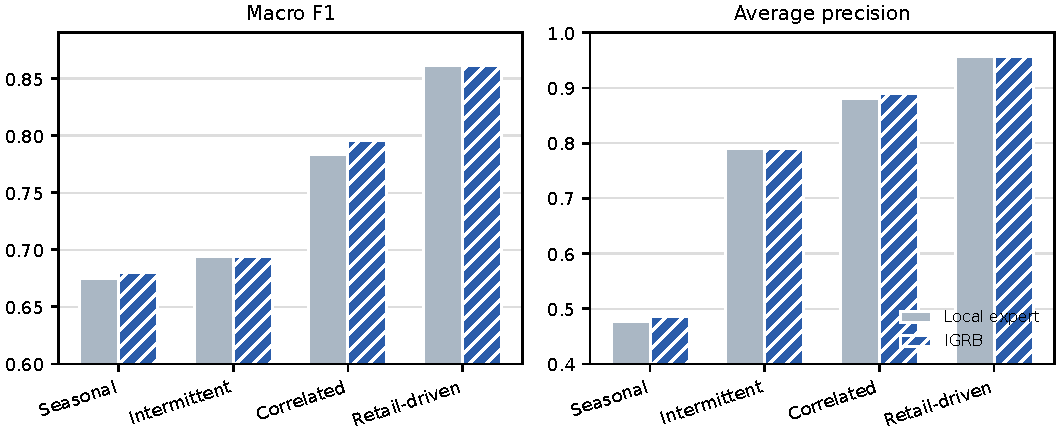
\includegraphics[width=.96\linewidth]{igrb_fixed_performance.pdf}
\caption{Fixed-realization occurrence performance, averaged over five model seeds. Exact ties occur where the intermittency screen returns IGRB to the local expert.}\label{fig:fixed}
\end{figure}

The independently sourced FMCG-inspired panel is reported separately because its source is simulated and only three parsimonious benchmark controls were rerun. IGRB improves over its tuned local expert but does not exceed standard XGBoost on macro F1. Its lower positive-severity RMSE shows a different occurrence--quantity trade-off rather than universal superiority.
\begin{table}[tb]\centering\small
\caption{FMCG-inspired robustness check under the unchanged condition (mean $\pm$ standard deviation over five model seeds; deterministic controls have zero standard deviation).}\label{tab:fmcg}
\begin{tabular}{lrrrr}\toprule Method & Macro F1 & AP & Brier & RMSE$^+$ \\\midrule
Local balance & $0.3682\pm0.0000$ & 0.1777 & 0.3998 & 12.0218 \\
Persistence & $0.7251\pm0.0000$ & 0.3392 & 0.1294 & 0.6154 \\
XGBoost & $0.7608\pm0.0003$ & 0.6345 & 0.0732 & 0.7799 \\
Tuned local expert & $0.7573\pm0.0025$ & 0.6322 & 0.0736 & 0.7376 \\
IGRB & $0.7592\pm0.0013$ & 0.6329 & 0.0737 & 0.6903 \\
\bottomrule\end{tabular}\end{table}
Against the strongest benchmark comparator, IGRB improves macro F1 in seasonal, intermittent and correlated demand and is practically tied in retail-driven demand. The intermittent gain is attributable to the retuned local expert because graph correction is disabled.
\begin{table}[tb]\centering\small
\caption{IGRB versus the strongest benchmark comparator, unchanged fixed realization.}\label{tab:previous}
\begin{tabular}{llrrr}\toprule Case & Previous best & Previous F1 & IGRB F1 & Difference \\\midrule
Seasonal & RelGRU & 0.6413 & 0.6804 & +0.0391 \\
Intermittent & LSTM & 0.6819 & 0.6939 & +0.0121 \\
Correlated & XGBoost & 0.7859 & 0.7953 & +0.0094 \\
Retail-driven & XGBoost & 0.8613 & 0.8611 & -0.0002 \\
\bottomrule\end{tabular}\end{table}
This comparison separates graph-specific gains from improvements in the local model. In seasonal and correlated demand, IGRB adds a nonzero graph correction and exceeds the strongest comparator by 0.0391 and 0.0094, respectively. In intermittent demand, its 0.0121 advantage over the strongest comparator comes entirely from the tuned local XGBoost reference. In retail-driven demand, the difference from the strongest XGBoost result is $-0.0002$, which is practically negligible and supplies no evidence of superiority.

Figure~\ref{fig:allbaselines} reports the complete fixed-realization comparison rather than only the strongest comparator. IGRB has the highest displayed mean in seasonal and correlated demand, ties its tuned local expert in intermittent demand, and is practically tied with both local XGBoost variants in the retail-driven case. The comparison also shows why the tuned local expert is a necessary reference: it is substantially stronger than several neural graph models, particularly on the retail-derived streams. Red outlines mark the column maximum or values within $5\times10^{-4}$ of it; they are descriptive fixed-record rankings, not significance claims.

\begin{figure}[tb]\centering
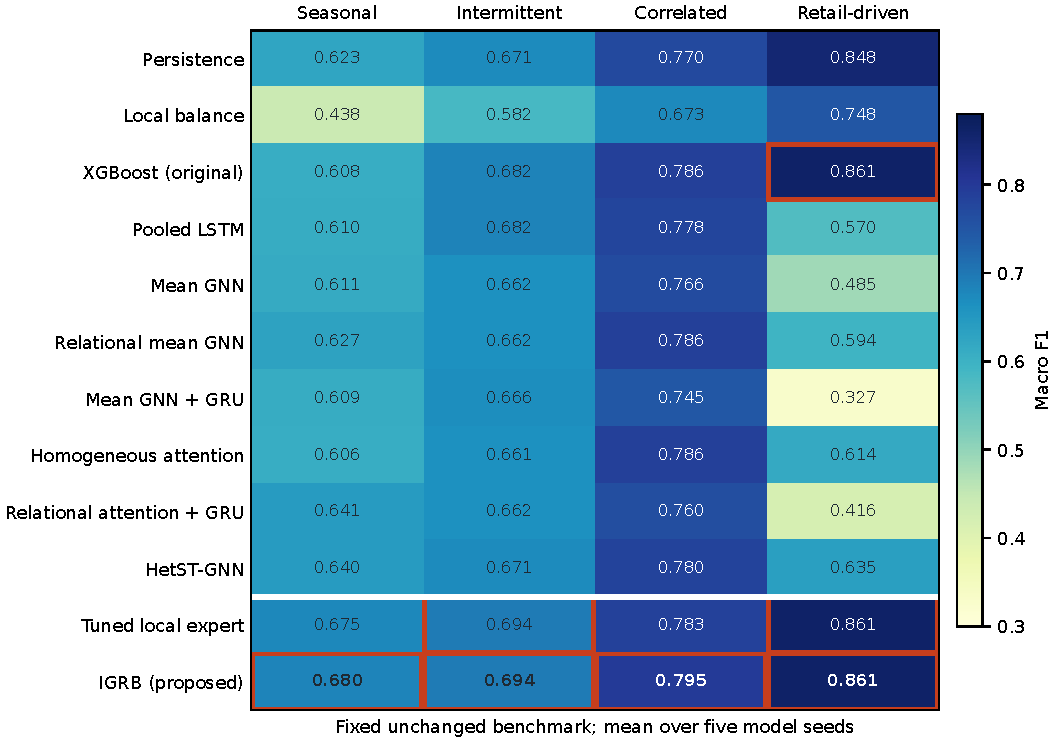
\includegraphics[width=.96\linewidth]{igrb_all_baselines.pdf}
\caption{Complete unchanged-condition macro-F1 comparison on the fixed benchmark realization. The first ten rows are benchmark methods; the last two rows are the tuned local reference and IGRB. Values are means over five model seeds, except deterministic controls. Red outlines denote the column maximum or a practical tie within 0.0005.}\label{fig:allbaselines}
\end{figure}
Independent records provide the stronger generalization check (Table~\ref{tab:independent}). The unchanged correlated-demand interval excludes zero across ten records; the seasonal interval crosses zero after five additional records are included. Intermittent demand is an exact fallback.
\begin{table}[tb]\centering\small
\caption{Paired IGRB minus local-expert macro-F1 differences over independent demand replications; percentile bootstrap intervals use 30,000 paired resamples.}\label{tab:independent}
\begin{tabular}{llrrrrr}\toprule Case & Condition & $n$ & Difference & 95\% interval & Wins & Losses \\\midrule
Seasonal & Unchanged & 10 & +0.0033 & [-0.0028, +0.0089] & 7 & 3 \\
Seasonal & Lead-time shift & 10 & -0.0087 & [-0.0278, +0.0087] & 4 & 6 \\
Seasonal & Policy shift & 10 & -0.0082 & [-0.0276, +0.0088] & 5 & 5 \\
\addlinespace
Intermittent & Unchanged & 5 & +0.0000 & [+0.0000, +0.0000] & 0 & 0 \\
Intermittent & Lead-time shift & 5 & +0.0000 & [+0.0000, +0.0000] & 0 & 0 \\
Intermittent & Policy shift & 5 & +0.0000 & [+0.0000, +0.0000] & 0 & 0 \\
\addlinespace
Correlated & Unchanged & 10 & +0.0269 & [+0.0080, +0.0436] & 9 & 1 \\
Correlated & Lead-time shift & 10 & +0.0149 & [-0.0083, +0.0358] & 8 & 2 \\
Correlated & Policy shift & 10 & +0.0228 & [+0.0094, +0.0420] & 9 & 1 \\
\addlinespace
\bottomrule\end{tabular}\end{table}
\begin{figure}[tb]\centering
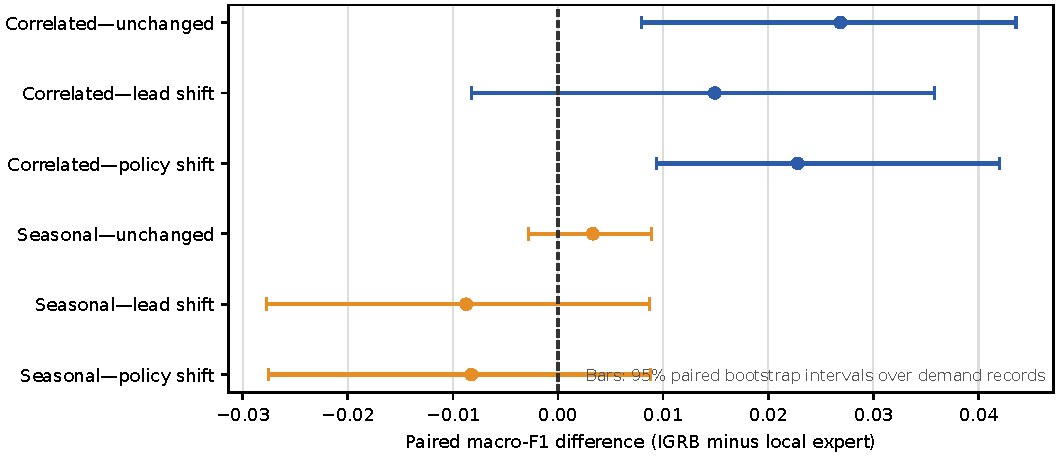
\includegraphics[width=.96\linewidth]{igrb_independent_effects.pdf}
\caption{Record-level paired effects after averaging five model seeds within each demand realization. The vertical reference is no difference; intervals are percentile paired-bootstrap intervals.}\label{fig:independent}
\end{figure}
The record-level evidence materially changes the conclusion suggested by the fixed benchmark. For unchanged correlated demand, the mean gain is 0.0269, nine of ten records favor IGRB and the interval remains above zero. Under the policy shift, nine of ten records also favor IGRB and the interval is positive. Under the lead-time shift, eight of ten favor it, but two adverse records widen the interval across zero. The appropriate claim is therefore robustness to unchanged and policy-shifted correlated demand, with uncertainty under longer transit time.

Seasonal demand is less stable. Seven of ten unchanged records favor IGRB, yet the mean gain is only 0.0033 and the interval spans zero. Under both shifts, the mean difference is negative and the intervals again span zero. The first five records were more favorable; the next five remove a broad seasonal-superiority conclusion. This is why demand-record uncertainty is reported separately from the small standard deviations over model seeds.
The component study in Table~\ref{tab:ablation} shows that forcing the graph expert harms intermittent demand and removing the ADI screen reduces its mean F1. Graph-only is slightly higher in the fixed dense cases, but it removes the fallback protection and its advantage is not evidence of general robustness. Error weighting is not uniformly beneficial and is excluded from the final method.
\begin{table}[tb]\centering\scriptsize
\caption{Component ablations on the unchanged fixed realization (mean $\pm$ standard deviation over five model seeds).}\label{tab:ablation}
\resizebox{\linewidth}{!}{\begin{tabular}{lrrrr}\toprule Case & Local only & Graph only & IGRB & Targeted ablation \\\midrule
Seasonal & 0.6752 $\pm$ 0.0035 & 0.6808 $\pm$ 0.0043 & 0.6804 $\pm$ 0.0037 & Error-weighted: 0.6808 $\pm$ 0.0050 \\
Intermittent & 0.6939 $\pm$ 0.0045 & 0.6851 $\pm$ 0.0035 & 0.6939 $\pm$ 0.0045 & No ADI: 0.6886 $\pm$ 0.0028 \\
Correlated & 0.7832 $\pm$ 0.0103 & 0.8051 $\pm$ 0.0084 & 0.7953 $\pm$ 0.0090 & Error-weighted: 0.7932 $\pm$ 0.0140 \\
Retail-driven & 0.8611 $\pm$ 0.0022 & 0.8625 $\pm$ 0.0013 & 0.8611 $\pm$ 0.0022 & No ADI: 0.8623 $\pm$ 0.0024 \\
\bottomrule\end{tabular}}\end{table}
The ablation also exposes the cost of a conservative method. Graph-only is 0.0099 above IGRB in the fixed correlated case and 0.0005 above it in seasonal demand. A method optimized solely for these two cells might therefore omit shrinkage and fallback. However, graph-only loses 0.0088 relative to local-only under intermittent demand, and the no-ADI variant also loses 0.0053 there. The selected design favors bounded downside across regimes over maximizing the best dense-case point estimate. In retail-driven demand, graph-only and no-ADI are slightly above the fallback point estimate, but the pre-specified ADI rule intentionally declines to treat that tiny fixed-record difference as sufficient evidence.

Table~\ref{tab:adi-sensitivity} tests whether this conclusion is an artifact of the borrowed 1.32 boundary. Cutoffs from 1.20 to 1.50 produce the same activation pattern and the same fixed-record results: graph correction is admitted for seasonal, correlated and FMCG-inspired demand and rejected for retail-driven and intermittent demand. A cutoff of 1.00 is too strict to admit the correlated and FMCG-inspired cases because their training ADIs are 1.007 and 1.143. At 2.00, the retail correction is admitted and adds only 0.0012 macro F1; intermittent demand, with ADI 2.549, still falls back. The analysis therefore supports a stable operating region rather than claiming that 1.32 is uniquely optimal.

\begin{table}[tb]\centering\scriptsize
\caption{Sensitivity of fixed-realization macro-F1 differences (selected framework minus local expert) to the ADI cutoff. S, C, F, R and I denote seasonal, correlated, FMCG-inspired, retail-driven and intermittent demand.}\label{tab:adi-sensitivity}
\resizebox{\linewidth}{!}{\begin{tabular}{lcrrrrr}\toprule
ADI cutoff & Graph-active cases & $\Delta$F1 S & $\Delta$F1 C & $\Delta$F1 F & $\Delta$F1 R & $\Delta$F1 I \\\midrule
1.00 & S & +0.0051 & +0.0000 & +0.0000 & +0.0000 & +0.0000 \\
1.20 & S, C, F & +0.0051 & +0.0120 & +0.0018 & +0.0000 & +0.0000 \\
1.32 & S, C, F & +0.0051 & +0.0120 & +0.0018 & +0.0000 & +0.0000 \\
1.50 & S, C, F & +0.0051 & +0.0120 & +0.0018 & +0.0000 & +0.0000 \\
2.00 & S, C, F, R & +0.0051 & +0.0120 & +0.0018 & +0.0012 & +0.0000 \\
\bottomrule\end{tabular}
}
\end{table}

The central operational result is the decision guardrail's selectivity, not the magnitude of one cost percentage. It abstains in seasonal, intermittent, retail-driven and FMCG-inspired cases even when a predictive score changes, preventing graph-based forecasts from automatically authorizing costly intervention. Only correlated demand clears the validation-cost conditions. There, IGRB lowers mean cost under all evaluated conditions (Table~\ref{tab:policy}); relative reductions are approximately 0.14\%, 1.27\% and 2.58\%. These are conditional simulator results, not universal policy superiority.
\begin{table}[tb]\centering\small
\caption{Correlated-demand closed-loop results (mean over five model seeds).}\label{tab:policy}
\begin{tabular}{lrrrr}\toprule Condition & Local cost & IGRB cost & Local fill & IGRB fill \\\midrule
Unchanged & 50907 & 50837 & 0.5796 & 0.5804 \\
Lead-time shift & 72665 & 71741 & 0.4637 & 0.4687 \\
Policy shift & 74467 & 72542 & 0.4379 & 0.4481 \\
\bottomrule\end{tabular}\end{table}
\begin{figure}[tb]\centering
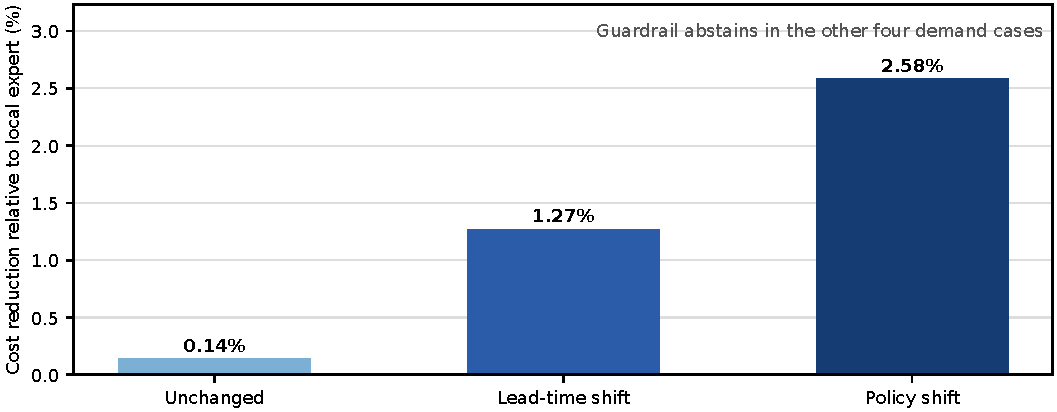
\includegraphics[width=.92\linewidth]{igrb_policy_savings.pdf}
\caption{Closed-loop cost reduction of the guarded IGRB policy relative to the guarded local-expert policy in correlated demand. Other cases are omitted because both guardrails abstain.}\label{fig:policy}
\end{figure}
The operational effect is smallest in the unchanged condition: cost falls by about 70 units out of 50,907 while fill rate rises from 0.5796 to 0.5804. This 0.14\% change is not presented as a large managerial saving. Its value is diagnostic: the complete forecast--selection--allocation pipeline avoids adding cost after the guardrail authorizes action. Under the lead-time shift the gap is about 923 units and fill rate rises by 0.0050; under the policy shift the gap is about 1,925 units and fill rate rises by 0.0102. These paired directional changes suggest more effective allocation of scarce emergency capacity in this simulated regime. They do not show that severity estimation is uniformly better, nor do they establish the optimality of the emergency rule.
\FloatBarrier


\section{Discussion}
The central finding is conditional. Network context is most useful when local histories omit a shared driver. The stable gain occurs in correlated demand: nine of ten unchanged records favor IGRB and the paired interval excludes zero. Under the policy shift the interval also excludes zero; under the lead-time shift it crosses zero. Seasonal unchanged and shifted intervals all cross zero after adding the confirmatory records. The initial five seasonal records were uniformly favorable, but the additional records remove that apparent certainty; reporting all ten avoids a seed-sensitive superiority claim.

\subsection{Why graph context helps selectively}
The correlated generator provides a mechanistic explanation for the strongest result. Terminals experience a shared latent log-intensity factor, but that factor is not included as a predictor. Parent, sibling and terminal histories provide multiple noisy measurements of its effect on orders, service and backlog. The graph-context expert can therefore recover information not fully summarized by the focal history. The improvement is not evidence that graphs are intrinsically superior; it is evidence that role-aligned context is useful when a shared driver is omitted locally.

Seasonality presents a weaker version of that mechanism. Calendar coordinates already expose the deterministic phase to the local expert, leaving less incremental information for other nodes. Neighbor states can still reveal realized common pressure or capacity effects, but the additional signal is small relative to record-to-record variation. This explains why the fixed realization improves while the ten-record interval includes zero. A larger model would not necessarily solve the issue: when incremental information is weak, additional capacity can increase selection variance.

Intermittency creates the opposite condition. Sparse nonzero arrivals mean that sibling and aggregate histories mix genuine inactivity with occasional bursts. Their short six-cycle windows can be poor estimates of a terminal's next active episode. The graph-only and no-ADI ablations show the resulting downside on the fixed intermittent record. Exact fallback is therefore a substantive part of the method, not merely a convenience for reporting ties.

The abstention mechanism is consequential. Intermittent and retail-driven cases have median ADI above the screen, so IGRB returns the local expert exactly. These are deliberate ties. The intermittent improvement over the former benchmark comes from retuning the local expert, not graph information. Graph-specific benefit is confined mainly to dense seasonal and correlated regimes.

The retail-driven fallback deserves particular caution. Graph-only is slightly higher than local-only on the fixed retail realization, so the ADI screen may forgo a small opportunity. But the case has one empirical demand panel, simulated operational states and no independent retail replications. Relaxing a pre-specified safeguard after observing a favorable point estimate would convert the screen into a post-hoc choice. The defensible conclusion is that the present evidence does not justify graph activation in this case. A future study could estimate an ADI boundary by nested validation across many industrial panels rather than borrowing 1.32.

\subsection{Prediction, severity and operational value}

Occurrence and severity do not improve uniformly. In seasonal demand, IGRB slightly reduces positive-target severity RMSE together with improving occurrence metrics. In correlated demand, it improves macro F1, AP and Brier score but increases severity RMSE. The closed-loop cost improvement there cannot be attributed to uniformly better quantity estimates; risk ranking, thresholds and the conservative allocation scale also matter.

This apparent tension is consistent with a capacity-limited policy. When the available emergency quantity cannot satisfy every predicted shortage, identifying which terminals should be served can matter more than accurately estimating every positive amount. Improved probability ranking can move scarce capacity toward the right terminals even if conditional quantities have larger average error. The policy scale of 0.25 also shrinks those quantities, limiting exposure to severity overestimation. Thus the cost result should be read as a property of the complete forecast--selection--allocation pipeline under the stated capacity, not as proof that both predictive heads improved.

The guardrail's abstentions provide negative operational evidence. Seasonal predictive improvements on the fixed record do not clear stable validation-cost requirements; intermittent and retail-driven predictions remain local and likewise do not justify purchases. Reporting only the correlated case could create the impression that emergency action is broadly beneficial. Reporting all abstentions makes the operational scope visible and supports a more realistic deployment pattern: use predictions for monitoring, but enable costly action only in regimes with repeatable validation benefit.

The guardrail chooses no action in seasonal, intermittent and retail-driven cases. In correlated demand, IGRB lowers mean cost relative to the local expert under unchanged, lead-time-shift and policy-shift conditions by approximately 0.14\%, 1.27\% and 2.58\%, respectively. Because these gains occur in one simulated regime with stylized costs and only five model seeds, they do not establish general inventory-control superiority.

The larger relative savings under the two shifts should not be interpreted as improved distributional robustness in general. Both shifts increase shortage pressure and therefore create more room for a constrained emergency channel to help. The policy shift retains a positive record-level predictive interval, whereas the lead-time interval crosses zero; nevertheless, mean closed-loop cost falls in both. This difference reinforces the need to evaluate decisions directly: a predictive confidence interval and an operational outcome answer different questions.

\subsection{Managerial interpretation}
The method suggests a three-stage implementation rule. First, maintain a strong local model as the default service. Second, activate network context only when training data are sufficiently dense and chronological validation shows incremental value. Third, treat action authorization as a separate governance decision with explicit costs, capacity and temporal stability checks. This structure is compatible with gradual deployment because each stage can abstain without breaking the forecasting pipeline.

The graph features also have operational meaning. A parent history represents replenishment availability; a sibling mean represents competition; a child mean represents downstream pressure; and a terminal aggregate represents common demand conditions. These summaries can be constructed from ordinary inventory records without requiring an end-to-end graph-learning platform. Their value depends on reliable timestamps and consistent node identifiers. In organizations where orders and receipts are recorded after decisions rather than when known, the feature timing must be revised to avoid leakage.

The results do not imply that managers should use 1.32 as a universal cutoff or adopt the simulated cost coefficients. Those values define a transparent experiment. In practice, the ADI gate should be estimated across historical panels with nested validation, and the action gate should use finance- and service-approved costs. A shadow-deployment period can record what the policy would have ordered while leaving existing operations unchanged, providing an initial external check of calibration, capacity use and intervention frequency.

\subsection{Validity threats and research agenda}

Limitations include one small tree, simulated shortage labels and states, a retail case with empirical demand only, and a borrowed ADI heuristic rather than a task-estimated boundary. Five independent replications do not cover topology uncertainty. The validation objective has fixed coefficients and the emergency rule is not jointly optimized. External validation should use timestamped industrial back orders, multiple networks, calibrated costs and nested validation of the intermittency boundary.

Internal validity depends on the simulator and event timing. Conservation tests reduce accounting errors, common random numbers support paired comparisons, and future-mutation tests address one class of leakage. They cannot prove that all implementation choices match a particular firm. Proportional allocation, one commodity, no substitution, fixed parent assignment and known uncensored demand simplify the system. Multi-sourcing, shared components, lost sales and supplier switching may change which graph roles are predictive.

Construct validity is limited by the chosen targets. A positive backlog two cycles ahead is useful for a two-cycle emergency channel, but it does not measure order lateness, customer priority or the duration of a shortage episode. Macro F1 weights both classes equally and AP emphasizes ranking; neither encodes monetary consequence. Conditional RMSE covers positive quantities but can be dominated by large shortages. The multi-metric report reduces dependence on one measure but does not eliminate the need for application-specific service outcomes.

External validity is the largest limitation. The retail source supplies demand traces only, and the synthetic cases intentionally isolate mechanisms rather than reproduce a population of supply chains. Ten records are enough to expose the fragility of the seasonal conclusion but not to characterize every demand distribution. Topology is fixed, and every node follows the same replenishment logic. Claims should therefore remain at the level of a controlled computational experiment until replicated on observed inventory, order, receipt, backlog and action logs from multiple networks.

Future work should prioritize evidence rather than architectural complexity. The first step is a multi-network dataset with decision-time snapshots and audit of when each variable became known. The second is nested estimation of the intermittency gate and blend objective across networks, leaving whole sites or product families out for external testing. The third is probability and severity calibration under shift, followed by a shadow-policy study using organization-specific costs. Only after these stages would joint optimization or a more expressive heterogeneous GNN be justified. Dynamic graph learning may be useful for supplier switching, but it should be compared with the same strong local and role-summary baselines.

\section{Conclusion}
IGRB converts network context from a mandatory representation into a validated residual correction. Validation controls correction strength, an intermittency screen permits exact fallback, and a separate guardrail controls intervention. Across independent realizations, the clearest gain is for correlated demand; seasonal evidence is mixed and intermittent demand triggers fallback. IGRB is competitive with the reconstructed benchmark in all cases, but decision-cost evidence remains conditional. The defensible conclusion is selective predictive value of graph context, not general graph-model or inventory-policy superiority.

\section*{Funding}This research received no external funding.
\section*{Data availability}
The only externally sourced dataset is UCI Online Retail, available under CC BY 4.0 at \url{https://doi.org/10.24432/C5BW33}. The seasonal, intermittent and correlated records are generated by the released simulator rather than downloaded from external repositories. Exact derived retail-demand matrices, synthetic generators, demand and simulator seeds, chronological split indices, per-run predictions and statistical summaries are included in the accompanying \texttt{IGRB\_Reproducibility\_Package.zip}. All inventory states, disruptions and back-order labels are simulated; the retail case uses empirical demand only. The supplementary package should be deposited in a permanent public repository and its archival DOI added to the submission metadata before external submission.
\section*{Code availability}
The accompanying reproducibility package contains the complete source, environment specification, run configurations, trained model artifacts, predictions, policy ledgers, tests and scripts used to regenerate all manuscript tables and figures, including the full-baseline comparison. \texttt{IGRB\_Zenodo\_Metadata.json} and \texttt{ZENODO\_UPLOAD\_CHECKLIST.md} are provided to support archival deposit. The historical record at \url{https://doi.org/10.5281/zenodo.22730609} predates this reconstruction and must not be cited as the source of the present numerical results.
\section*{Declaration of competing interests}The authors declare no known competing financial interests or personal relationships that could have appeared to influence this work.

\begin{thebibliography}{99}
\bibitem{clark} A. J. Clark and H. Scarf. Optimal policies for a multi-echelon inventory problem. \emph{Management Science} 6(4), 475--490, 1960. \url{https://doi.org/10.1287/mnsc.6.4.475}.
\bibitem{graves} S. C. Graves and S. P. Willems. Optimizing strategic safety stock placement in supply chains. \emph{Manufacturing \& Service Operations Management} 2(1), 68--83, 2000. \url{https://doi.org/10.1287/msom.2.1.68.23267}.
\bibitem{gardner} E. S. Gardner Jr. Evaluating forecast performance in an inventory control system. \emph{Management Science} 36(4), 490--499, 1990. \url{https://doi.org/10.1287/mnsc.36.4.490}.
\bibitem{kolassa} S. Kolassa. Evaluating predictive count data distributions in retail sales forecasting. \emph{International Journal of Forecasting} 32(3), 788--803, 2016. \url{https://doi.org/10.1016/j.ijforecast.2015.12.004}.
\bibitem{spo} A. N. Elmachtoub and P. Grigas. Smart ``Predict, then Optimize''. \emph{Management Science} 68(1), 9--26, 2022. \url{https://doi.org/10.1287/mnsc.2020.3922}.
\bibitem{trees} A. N. Elmachtoub, J. C. N. Liang and R. McNellis. Decision trees for decision-making under the predict-then-optimize framework. \emph{ICML}, PMLR 119, 2858--2867, 2020. \url{https://proceedings.mlr.press/v119/elmachtoub20a.html}.
\bibitem{mandi} J. Mandi, V. Bucarey, M. M. K. Tchomba and T. Guns. Decision-focused learning: Through the lens of learning to rank. \emph{ICML}, PMLR 162, 14935--14947, 2022. \url{https://proceedings.mlr.press/v162/mandi22a.html}.
\bibitem{gcn} T. N. Kipf and M. Welling. Semi-supervised classification with graph convolutional networks. \emph{ICLR}, 2017. \url{https://arxiv.org/abs/1609.02907}.
\bibitem{rgcn} M. Schlichtkrull, T. N. Kipf, P. Bloem, R. van den Berg, I. Titov and M. Welling. Modeling relational data with graph convolutional networks. \emph{ESWC}, 593--607, 2018. \url{https://doi.org/10.1007/978-3-319-93417-4_38}.
\bibitem{gat} P. Veli\v{c}kovi\'{c}, G. Cucurull, A. Casanova, A. Romero, P. Li\`o and Y. Bengio. Graph attention networks. \emph{ICLR}, 2018. \url{https://arxiv.org/abs/1710.10903}.
\bibitem{dcrnn} Y. Li, R. Yu, C. Shahabi and Y. Liu. Diffusion convolutional recurrent neural network: Data-driven traffic forecasting. \emph{ICLR}, 2018. \url{https://openreview.net/forum?id=SJiHXGWAZ}.
\bibitem{stgcn} B. Yu, H. Yin and Z. Zhu. Spatio-temporal graph convolutional networks: A deep learning framework for traffic forecasting. \emph{IJCAI}, 3634--3640, 2018. \url{https://doi.org/10.24963/ijcai.2018/505}.
\bibitem{graphwavenet} Z. Wu, S. Pan, G. Long, J. Jiang and C. Zhang. Graph WaveNet for deep spatial-temporal graph modeling. \emph{IJCAI}, 1907--1913, 2019. \url{https://doi.org/10.24963/ijcai.2019/264}.
\bibitem{mtgnn} Z. Wu, S. Pan, G. Long, J. Jiang, X. Chang and C. Zhang. Connecting the dots: Multivariate time series forecasting with graph neural networks. \emph{KDD}, 753--763, 2020. \url{https://doi.org/10.1145/3394486.3403118}.
\bibitem{xgb} T. Chen and C. Guestrin. XGBoost: A scalable tree boosting system. \emph{KDD}, 785--794, 2016. \url{https://doi.org/10.1145/2939672.2939785}.
\bibitem{m4} S. Makridakis, E. Spiliotis and V. Assimakopoulos. The M4 Competition: 100,000 time series and 61 forecasting methods. \emph{International Journal of Forecasting} 36(1), 54--74, 2020. \url{https://doi.org/10.1016/j.ijforecast.2019.04.014}.
\bibitem{m5} S. Makridakis, E. Spiliotis and V. Assimakopoulos. The M5 accuracy competition: Results, findings, and conclusions. \emph{International Journal of Forecasting} 38(4), 1346--1364, 2022. \url{https://doi.org/10.1016/j.ijforecast.2021.11.013}.
\bibitem{deepar} D. Salinas, V. Flunkert, J. Gasthaus and T. Januschowski. DeepAR: Probabilistic forecasting with autoregressive recurrent networks. \emph{International Journal of Forecasting} 36(3), 1181--1191, 2020. \url{https://doi.org/10.1016/j.ijforecast.2019.07.001}.
\bibitem{nbeats} B. N. Oreshkin, D. Carpov, N. Chapados and Y. Bengio. N-BEATS: Neural basis expansion analysis for interpretable time series forecasting. \emph{ICLR}, 2020. \url{https://openreview.net/forum?id=r1ecqn4YwB}.
\bibitem{tft} B. Lim, S. O. Arik, N. Loeff and T. Pfister. Temporal Fusion Transformers for interpretable multi-horizon time series forecasting. \emph{International Journal of Forecasting} 37(4), 1748--1764, 2021. \url{https://doi.org/10.1016/j.ijforecast.2021.03.012}.
\bibitem{batesgranger} J. M. Bates and C. W. J. Granger. The combination of forecasts. \emph{Operational Research Quarterly} 20(4), 451--468, 1969. \url{https://doi.org/10.2307/3008764}.
\bibitem{clemen} R. T. Clemen. Combining forecasts: A review and annotated bibliography. \emph{International Journal of Forecasting} 5(4), 559--583, 1989. \url{https://doi.org/10.1016/0169-2070(89)90012-5}.
\bibitem{croston} J. D. Croston. Forecasting and stock control for intermittent demands. \emph{Operational Research Quarterly} 23(3), 289--303, 1972. \url{https://doi.org/10.1057/jors.1972.50}.
\bibitem{sba} A. A. Syntetos and J. E. Boylan. The accuracy of intermittent demand estimates. \emph{International Journal of Forecasting} 21(2), 303--314, 2005. \url{https://doi.org/10.1016/j.ijforecast.2004.10.001}.
\bibitem{tsb} R. H. Teunter, A. A. Syntetos and M. Z. Babai. Intermittent demand: Linking forecasting to inventory obsolescence. \emph{European Journal of Operational Research} 214(3), 606--615, 2011. \url{https://doi.org/10.1016/j.ejor.2011.05.018}.
\bibitem{syntetos} A. A. Syntetos, J. E. Boylan and J. D. Croston. On the categorization of demand patterns. \emph{Journal of the Operational Research Society} 56(5), 495--503, 2005. \url{https://doi.org/10.1057/palgrave.jors.2601841}.
\bibitem{brier} G. W. Brier. Verification of forecasts expressed in terms of probability. \emph{Monthly Weather Review} 78(1), 1--3, 1950. \url{https://doi.org/10.1175/1520-0493(1950)078<0001:VOFEET>2.0.CO;2}.
\bibitem{sargent} R. G. Sargent. Verification and validation of simulation models. \emph{Journal of Simulation} 7(1), 12--24, 2013. \url{https://doi.org/10.1057/jos.2012.20}.
\bibitem{gama} J. Gama, I. \v{Z}liobait\.{e}, A. Bifet, M. Pechenizkiy and A. Bouchachia. A survey on concept drift adaptation. \emph{ACM Computing Surveys} 46(4), Article 44, 2014. \url{https://doi.org/10.1145/2523813}.
\bibitem{chang} S. Chang et al. Learning production functions for supply chains with graph neural networks. arXiv:2407.18772, version 3, 2025. \url{https://arxiv.org/abs/2407.18772}.
\bibitem{kotecha} N. Kotecha and A. del Rio Chanona. Leveraging graph neural networks and multi-agent reinforcement learning for inventory control in supply chains. arXiv:2410.18631, version 2, 2025. \url{https://arxiv.org/abs/2410.18631}.
\bibitem{uci} D. Chen. Online Retail [Dataset]. UCI Machine Learning Repository, 2015. \url{https://doi.org/10.24432/C5BW33}.
\end{thebibliography}\end{document}
